\chapter{Introduction}
\label{sec:in}

\section{Background}
The link between degeneracy in biological systems and structural unidentifiability in parameter models.

\subsection{Degeneracy in Biological Systems}
Cellular homeostasis mechanisms allow a neuron to maintain a functional target pattern in the presence of changes in their membrane properties and electrical activity. Homeostatic regulation is thus associated with stable neuronal activity which enables the brain with the necessary reliability  in order to perform their functions properly. By contrast, the capabilities of the brain to learn, store memory and adapt to changes in the environment are associated with certain network plasticity which lead to changing and dynamical synapses between neurons. Together with cellular homeostasis mechanisms, it has been suggested some synaptic homeostasis mechanisms, such as synaptic scaling, which prevent the network to become unstable and, at the same time, they allow plastic changes \cite{Astrid}. Moreover, homeostatic regulation mechanisms at the network level has also been reported. 

Among homeostatic regulation mechanisms, it is the activity-dependent homeostatic regulation (ADHR) mechanism. It constitutes a negative feedback system through which neurons are able to restore their properties and compensate changes due to external perturbations \cite{Astrid}. It allows neurons to maintain the so-called target activity level or functional activity.

Neuronal and network properties need to be constrained in order to achieve the target neural behavior of any activity-dependent homeostatic mechanism, both at the neuron and network level. Usually, these constraints result in regions on parameter space which generate a desired neuron behavior. When this target activity level is characterized by certain attributes, attribute LSs can represent these regions. The fact that a wide range of parameter combinations can generate the same neuron output make neurons more robust to perturbations.

The idea that target activity levels can be achieved with different parameters combinations, instead of having to tune parameters to specific unique values has experimental evidence. In \cite{Swensen3509}, they show how the value of two currents were different in cells showing almost identical electrical activity patterns, Fig. (\ref{photonew1}) .

\begin{figure}[htb]
\centering
    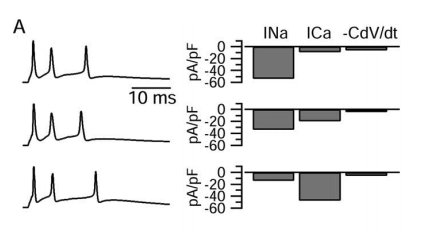
\includegraphics[width=0.7\linewidth]{Images/photonew1.png} 
  \caption{\textbf{Similar neuron activity with different values of sodium and calcium currents.} Left: similar voltage traces of three different neurons. Right: bar plots showing the value of the sodium ($I_{Na}$) and calcium ($I_{Ca}$) current for each neuron. It is also shown the net current through the membrane ($-CdV/dt$). Figure taken from \cite{Swensen3509}.}
  \label{photonew1}
\end{figure}

Moreover the so-called animal-to-animal parameter variability, consisting on parameter differences on a given neuron type from animal to animal, also supports the idea \cite{Schulz2006}. Several-fold variations in conductance densities from one animal to another have been reported.

Theoretical work using computational models has also shown that similar network activity can be generated with several combinations of synaptic strengths and intrinsic properties \cite{Prinz}. In this work, a three-cell (AB/PD-LP-PY) network model for the pyloric network of the crustacean stomatogastric ganglion (STG) was used to show that different sets of synaptic and intrinsic parameters give rise to similar network activity, Fig. (\ref{photonew3}).

\begin{figure}[htb]
\centering
    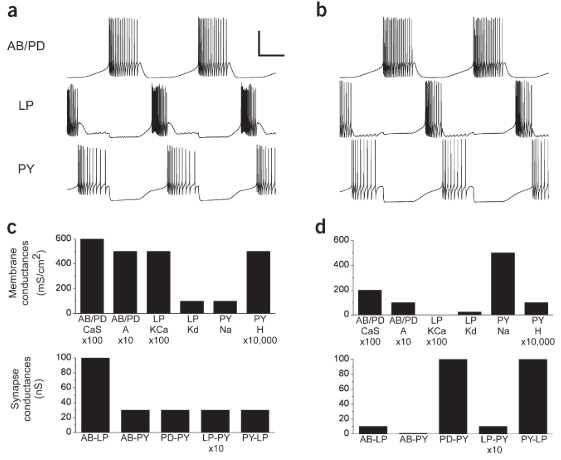
\includegraphics[width=0.8\linewidth]{Images/photonew3.png} 
  \caption{\textbf{Similar pyloric rhythms from different networks.} Top: voltage traces for each cell type (AB/PD, LP and PY) for two different networks. Bottom: parameter values of several membrane and synaptic parameters. To one network it corresponds plots (a)-(c). Plots (b)-(d) correspond to the other network. Figure taken from \cite{Prinz}}
  \label{photonew3}
\end{figure}

Furthermore, neuronal parameters seem not to vary independently among different solutions on parameter space for the same neuronal target, but it seems that there are dependencies among parameters producing parameter correlations \cite{Khorkova8709}.

\subsection{Parameter Estimation Unidentifiability}

Parameter variability must be taken into account on model construction, when it is intended to replicate experimental observations. Since only a small fraction of neuron properties are experimentally available, experimentally non-accessible parameters need to be determined and fit to experimental data. The ability of the models to make predictions and to provide mechanistic explanations depends on the reliability of this process.

Neuronal parameter optimization is the process of identifying sets of parameters that lead to a desired electrical activity pattern in a neuron or neuronal network model that is not fully constrained by experimental data \cite{sc}. In order to perform this process, a large number of parameter estimation techniques (PE) and tools are available to scientist, which involve hand-tuning, optimization methods, such as the gradient method, or parameter space explorations techniques \cite{sc1}. A key feature of these methods is a measure, which indicates how well the model is able to produce the desired electric target. Parameter sets which acceptably reproduce the desired electrical activity are called the solutions for the optimization problem. When there are  multiple solutions for an optimization problem, the set of solution is known as the “solution space” of the problem \cite{sc1}.

The fact that the target activity level of a neuron is presumably an electrical activity pattern rather than specific set of parameters on a given model, give rise to the degeneracy problem. Degeneracy refers to the situations where multiple sets of parameters values can produce the same observable output, therefore making the inverse problem ill-posed, i.e., determining the model parameters from observable experimental data is not a well-defined problem.

Two sources account for parameters to be unidentifiable: structural and practical unidentifiability. Practical identifiability is related to experimental/noisy data. One can at best expect to estimate distribution of parameters around a "true" mean. 

Structural identifiability refers to the problem of whether it is possible to uniquely determine the unknown model parameters from a set of observable outputs. It is only based on the inherent structure of a given model and it is the type of unidentifiability of interest to this project since it is thought to have a direct connection with biological degeneracy and homeostatic regulation processes.

Several techniques are available the for analysis of structural identifiability, specially in linear ODE models \cite{GODFREY198589}. Furthermore more recent methods have been proposed for general non-linear ODE models \cite{sc2}. Although the increasing difficulty of these methods as models become more complex, the structural identifiability analysis should be investigated in any parameter identification problem. 

The general framework in which structural identifiability is performed involve a dynamical system model of the form
\begin{equation}
    \dot{x}(t) = f(x(t),t,u(t),\theta), \hspace{0.5cm} x(t_{0})=x_{0}
    \label{1}
\end{equation}
\begin{equation}
    y(t) = h(x(t),t,\theta)
    \label{2}
\end{equation}
where $x(t)$ represent state variables, $t$ is the time, $u(t)$ is a given input, $\theta$ represent model parameters and $y(t)$ is the output (measurements/observations). Initial conditions are given by $x_{0}$.

Mathematically, considered a system of the form Eqs. (\ref{1})-(\ref{2}), a given individual parameter set $\theta$ is said to be structurally identifiable, \cite{Eisenberg2014}, if for almost every set of parameters $\bar{\theta}$ and almost all initial conditions
\begin{equation}
    y(x(t),t,\bar{\theta}) = y(x(t),t,\theta) \Longrightarrow \bar{\theta} = \theta
\end{equation}
Otherwise, the system model is said to be structurally unidentifiable. Typically, unidentifiable model parameters form identifiable combinations, which consist in set of parameters which can be identifiable as a set \cite{Eisenberg2014}.

All considered, the biological consequences of homeostatic regulation mechanisms not only at the neuron level, but also at a network level involving synaptic connections, make the model construction task quite challenging. 

On the one hand, the physiological parameter variability must be reflected in the model. From a mathematical perspective, attribute level sets must show properties in accordance to the biology beyond these mathematical structures. The study of attribute level sets in single neuron and network models try to shed light on this issue. 

On the other hand, the ability of models to make predictions and to provide mechanistic explanations depends on how reliable model parameters are tuned in order to reflect realistic cellular and network behavior based on experimental attribute measurements. Degeneracy of biological systems, which seem to be inherent to the biology nature, imposes several difficulties on this process. 


\section{Significance}
Some parameter estimation techniques, such as parameter space exploration techniques, are aware of the structural unidentifiability of neuron and network models and focus on finding regions on parameter space with a desired neuron or network activity. Those model scan the parameter space producing the so-called “model databases”, which provide valuable information of how parameters could be homeostatically regulated in order to produce a target activity \cite{Prinz2007}. When a target behavior is characterized by the value of certain attributes, attribute level sets appear. They represent point on parameter space for which a given attribute is constant, i.e., manifolds on parameter space preserving a given attribute value. If a neural or network activity target is characterized by several attributes values, the intersection of their corresponding manifolds represents the region on parameter space preserving all attributes values characterizing the activity target.

Among the disadvantages of these method, it is the high computational cost and the exponentially increase in number of simulations as the parameter space is extended, which is usually required in neural networks. Moreover methods are mainly qualitative. In this respect, the study of basic level sets properties in simple single neuronal and network models can help in the understanding of how homeostatic rules are linked with attribute level sets.

\section{Project Design}
The goal of the project is to study how individual neuron LSs are behaved when cells become part of a network. We ask whether and under what conditions individual attribute LSs are preserved in a network structure and how new network level sets emerge.

An oversimplified single neuron model is used to represent the behavior of a single cell. Characterizing degeneracy is this simple model, we are able to find conditions on connectivity parameter space for the preservation of individual level sets.  When these conditions are not guaranteed, new network level sets emerge on parameter spaces which might involve both connectivity and intrinsic parameters from single cells. We consider networks with  different degree of complexity based on individual intrinsic parameters, distinguishing between homogeneous and heterogeneous networks and compare LSs properties between them. 

\section{Project Information}
Part of this project was selected for The Virtual Dana Knox Student Research Showcase (New Jersey Institute of Technology).

The full project has also been chosen for a poster presentation at the Organization for Computational Neuroscience (CNS) annual meeting (2021). Fig. (\ref{photonew33}) shows the poster of this project for the meeting.

\begin{figure}[htb]
\centering
    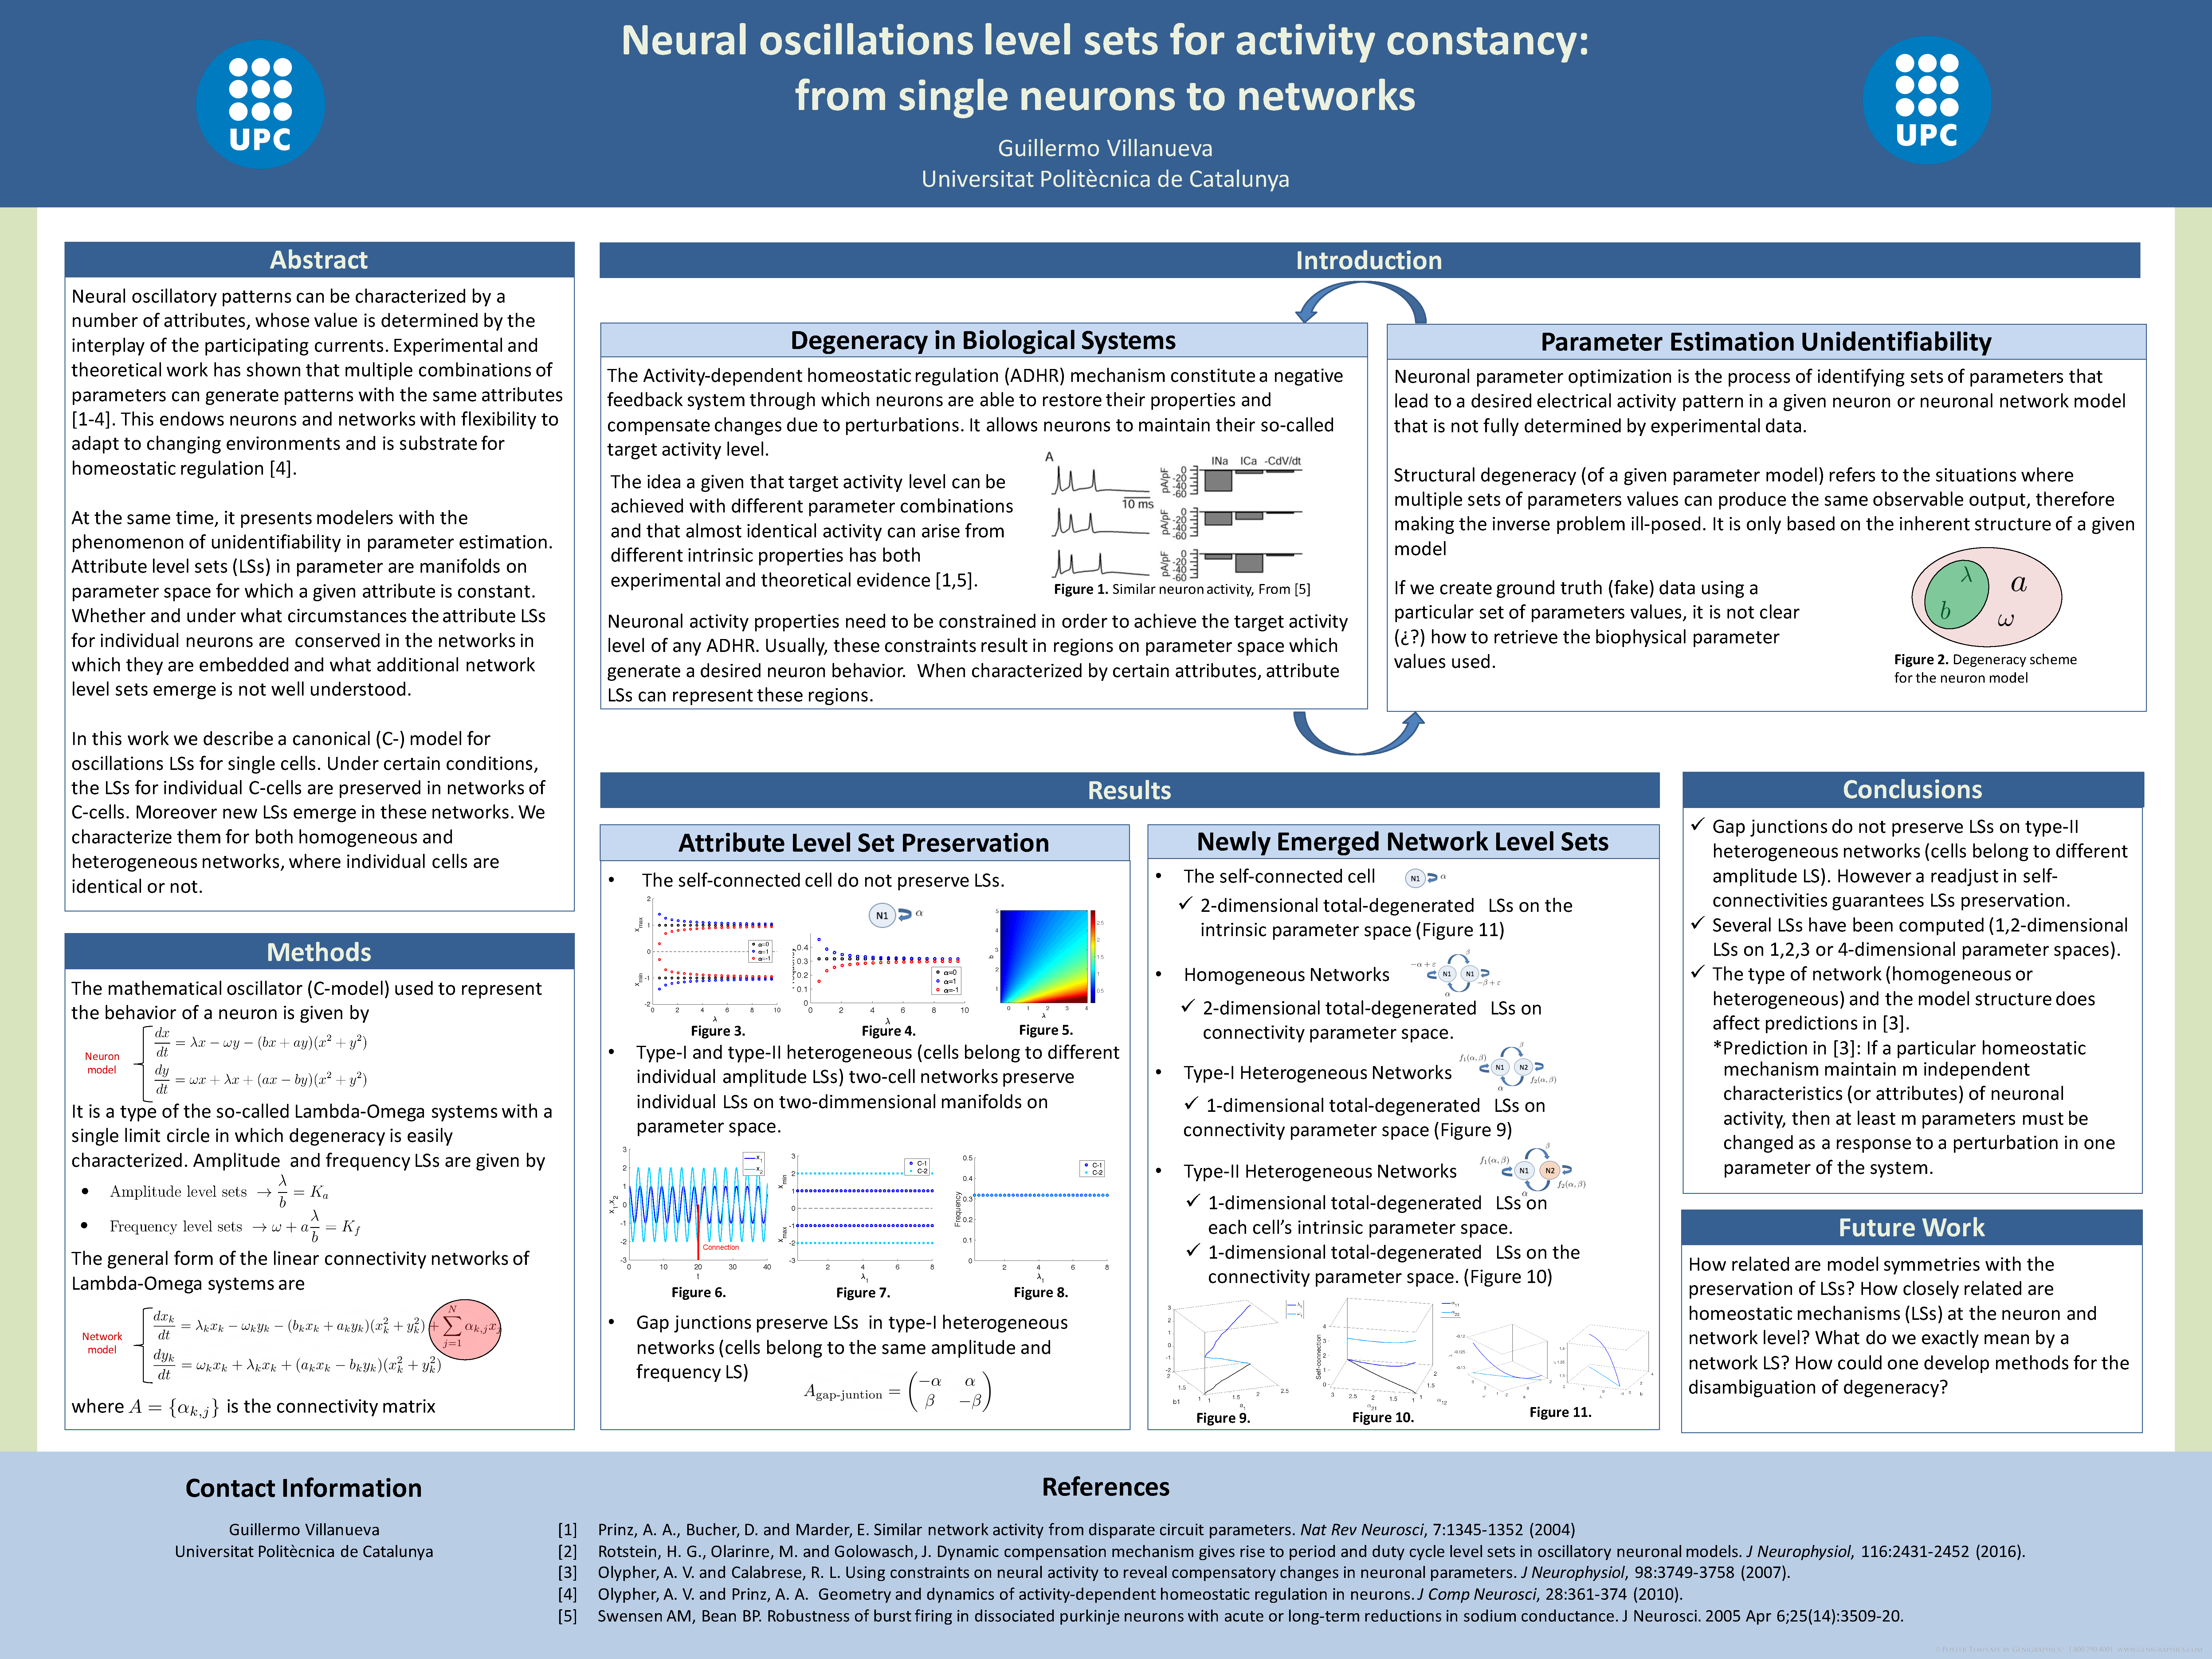
\includegraphics[width=1\linewidth]{Images/poster.pdf} 
  \caption{\textbf{Poster for the CNS 2021 annual meeting.}}
  \label{photonew33}
\end{figure}

\section{Project Overview}

\begin{itemize}

    \item \textbf{Chapter 1: Introduction.} It is this chapter. The significance of the project is stated, for which some background on the field is given. It is also given a summary of the project and an overview of the thesis section by section.
    
    \item \textbf{Chapter 2: Background.} Theoretical background on computational neuroscience in the context of this work is presented. The section gives an overview of basic single neuron and synaptic dynamics model. Furthermore some mathematical models for neuronal networks are presented. Some concepts are illustrated on a realistic biophysical network model of the basal ganglia.
    
    \item \textbf{Chapter 3: Previous work.} Review of previous work related with attribute level sets. Two papers and one PhD rotation project are mainly summarized. 
    
    \item \textbf{Chapter 4: Methods.} This section introduces the single neuron model, as well as, the type of networks considered in this work. Furthermore, degeneracy is characterized in this single neuron model. In addition, important concepts for following sections are defined.
    
    \item \textbf{Chapter 5: Level Sets Preservation in $\Lambda \Omega_{2}-$Networks.} Results are presented. They include conditions for the preservation of level sets in two-cell networks.
    
    \item \textbf{Chapter 6: Newly Emerged Network Level Sets.} Results are presented. Systematic qualitative study of the newly emerged network level sets both in the self-connected cell and the two-cell network.
    
    \item \textbf{Chapter 7: Discussion.} Final summary of the work, in which results are discussed and new lines of research are mentioned. Moreover a personal conclusion is done. 
    
\end{itemize}
Two appendices are also included:    
\begin{itemize}

    \item \textbf{Appendix A: On Level Sets Preservation.} Mathematical derivation for level sets preservation in the two-cell network. The appendix supports Chapter 5.
    
    \item \textbf{Appendix B: Codes.} Some representative (non-exhaustive) set of files used in this project are shown.

\end{itemize}

    

